\documentclass[a4paper,12pt]{article}
\usepackage[utf8]{inputenc}
\usepackage[russian]{babel}
\usepackage{array}
\usepackage[left=20mm,top=20mm,right=20mm,bottom=20mm]{geometry}
\usepackage{tabularx}
\usepackage{longtable}
\usepackage[pdftex]{graphicx}
\usepackage{xcolor}
\usepackage{textcomp}
\usepackage{amssymb}
\usepackage{hyperref}
\usepackage{soul}
\usepackage{listings}
\usepackage{cite}
\usepackage{amsmath}
\usepackage{float}

%opening
\title{Qucs-S: Simulation reference}
\author{Vadim Kuznetsov}

\begin{document}

\maketitle

\tableofcontents

\listoffigures

\listoftables

%\begin{abstract}

%\end{abstract}

\clearpage
\section{Введение} \label{sec:intro}

\subsection{Общие сведения}

Qucs-S является форком проекта Qucs, который начали разрабатывать Stefan Jahn и Michael Margraf из Берлинского института высокочастотной техники в 2003 году. Изначально Qucs поставлялся со своим собственным движком моделирования, нацеленным более на анализ ВЧ схем в частотной области. Этот движок имел серьёзные проблемы со сходимостью при моделировании во временной области  и был несовместим со SPICE, что не позволяло напрямую применять модели электронных компонентов, распространяемые производителями.

В 2014 году была начата разработка набора патчей, который бы позволял подключать к Qucs в качестве движка открытый Ngspice. В итоге эта разработка привела к созданию форка Qucs-S (Qucs with SPICE). В настоящее время Qucs-S представляет собой самостоятельный программный продукт для моделирования аналоговых электронных схем общего назначения. 

\subsection{Руководство по установке Qucs-S}

Для Linux имеются репозитории для Debian/Ubuntu, Fedora и OpenSUSE. Имеются также пакеты для Arch, которые можно установить через AUR, и порт для FreeBSD. Для нестандартных случаев можно собрать Qucs-S из исходников или воспользоваться AppImage. Поддержку своего дистрибутива Linux можно проверить здесь:  \url{https://download.opensuse.org/repositories/home:/ra3xdh/} Бинарные пакеты собираются автоматически при помощи OpenSUSE Build Service. 

Сам Qucs-S не предоставляет движка моделирования, кроме QucsatorRF. Рекомендуется использовать Ngspice, который для Debian/Ubuntu устанавливается по зависимостям, а в прочих случаях его нужно установить вручную. 

Движок QucsatorRF входит в состав бинарных пакетов начиная с версии 24.2.0. Устанавливать его отдельно не требуется.

Для Windows существуют два варианта бинарных пактов: инсталлятор и zip-архив с portable версией. Второй вариант рекомендуется если воспользоваться инсталлятором невозможно по причине отсутствия административных прав. Инсталлятор включает в себя бинарную версию Ngspice. Установка при помощи инсталлятора особенностей не имеет. Следует запустить исполняемый файл и следовать инструкциям. Затем следует запустить Qucs-S из меню "Пуск". Программа обнаруживает установленный вместе с ней Ngspice автоматически.

Чтобы установить portable версию нужно распаковать ZIP архив и запустить файл \verb|qucs-s.exe| из поддиректории \verb|bin|. Ngspice следует скачать с официального сайта \url{http://ngspice.sourceforge.net/}. При первом запуске следует указать путь к файлу -- \verb|ngspice_con.exe| в настройках программы. 



\section{Моделирование с движком SPICE}

\subsection{Поддерживаемые движки моделирование и быстрое переключение симуляторов}

В настоящее время Qucs-S поддерживает четыре движка моделирования:

\begin{itemize}
 \item Ngspice \url{http://ngspice.sourceforge.net/} Это рекомендованный симулятор. Он совместим с большинством моделей, предоставляемых производителями электронных компонентов и открытыми PDK для разработки ИМС;
 \item XYCE \url{https://xyce.sandia.gov/} Это симулятор разработанный Сандийскими национальными лабораториями. Имеется возможность моделирования гармонического баланса (HB) и S-параметров;
 \item Qucsator \url{https://github.com/ra3xdh/qucsator_rf} имеет возможность моделирования S-параметров и расширенный набор ВЧ компонентов в том числе микрополосковых линий. Не является SPICE совмесмым и не рекомендуется для анализа схем общего назначения;
 \item SpiceOpus \url{http://www.spiceopus.si/}
\end{itemize}

Особенностью Qucs-S является то, что этот симулятор позволяет выбирать между несколькими движками моделирования. Движком по умолчанию начиная с версии 0.0.23 предлагается Ngspice, который лучше всего подходит для моделирования любых электронных схем. Всего в Qucs-S доступно три движка моделирования. Qucsator, который был движком по умолчанию в старом Qucs, содержит расширенный набор компонентов для анализа СВЧ устройств, таких как модели волноводов и микрополосковых линий. Но использовать Qucsator для моделирования схем общего назначения не рекомендуется по причине отсутствия совместимости со SPICE и нестабильной работы на схемах с импульсными воздействиями. 

В Qucs-S начиная с версии 2.0.0 можно переключаться между движками моделирования на ходу без перезагрузки программы. Для этого рядом с кнопкой запуска симуляции на панели инструментов добавлен выпадающий список (рис. \ref{fig:sim_switch}), из которого можно выбрать симулятор. При этом компоненты на левой панели будут автоматически перезагружены, и остаются только совместимые с выбранный движком. Несовместимые компоненты также помечаются в самой схеме. 

    \begin{figure}[!ht]
    \begin{center}
        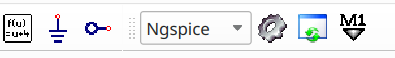
\includegraphics[width=0.5\textwidth]{img/sim_switch.png}
    \end{center}
    \caption{Выпадающий список выбора симулятора} \label{fig:sim_switch}
    \end{figure}

\subsection{Расчёт рабочей точки на постоянном токе}

Расчёт рабочей точки по постоянному току позволяет рассчитать напряжение и ток в узлах и компонентах схемы в установившемся режиме при условии отсутствия входного сигнала переменного тока. Чтобы запустить расчёт рабочей точки, нужно в главном меню Qucs-S выбрать \emph{Simulation->Calculate DC bias} или нажать клавишу F8 на клавиатуре. Если схема собрана без ошибок, то рядом с узлами схемы программа покажет значение напряжения, а рядом с источниками – величину тока, протекающего через этот источник. В схему также можно включать вольтметры и амперметры.


    \begin{figure}[!ht]
    \begin{center}
        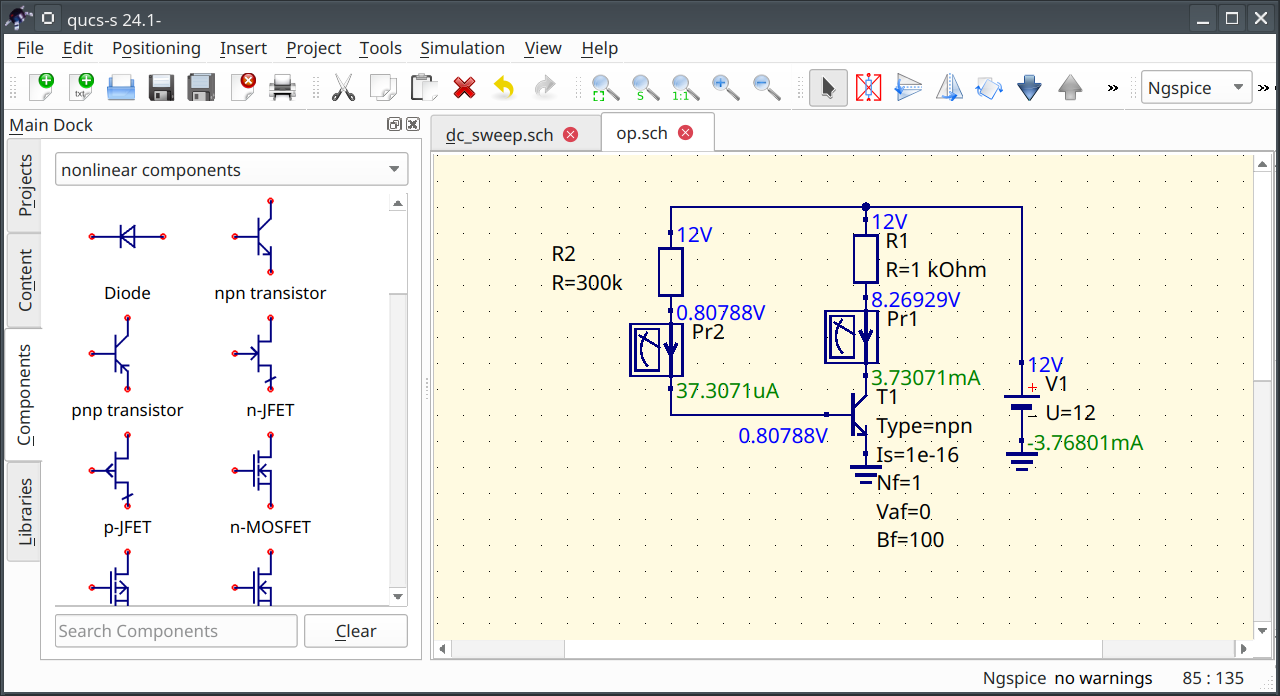
\includegraphics[width=\textwidth]{img/dc_f8.png}
    \end{center}
    \caption{Моделирование рабочей точки} \label{fig:dc_f8}
    \end{figure}
    
На рис. \ref{fig:dc_f8} показан  пример моделирования рабочей точки простой схемки на биполярном транзисторе. В цепь коллектора и в цепь базы включены амперметры. Использована идеальная модель транзистора с коэффициентом передачи тока Bf=100.  Из результатов моделирования видно, что ток коллектора примерно в Bf раз больше, чем ток базы.

\subsection{Моделирование на постоянном токе}

Моделирование на постоянном токе (DC sweep) позволяет также рассчитать напряжение и ток в узлах и компонентах схемы в установившемся режиме при условии отсутствия входного сигнала переменного тока. Но при этом можно построить зависимость выходного сигнала от некоторого напряжения, тока или сопротивления. В числе возможных применений данного моделирования – построение вольт-амперных характеристик (ВАХ) полупроводниковых и электровакуумных приборов. 

В качестве примера рассмотрим как промоделировать выходную ВАХ полевого транзистора. Как известно выходная ВАХ -– это зависимость тока стока $I_d$ транзистора от напряжения сток-исток $V_{ds}$ при постоянном напряжении смещении на затворе $V_{gs}$. Как правило в справочниках приводится семейство выходных ВАХ для различного напряжения на затворе. Чтобы провести моделирование, в Qucs-S собираем схему (рис. \ref{fig:dc_sweep}), содержащую транзистор, два источника, и виды моделирования.

    \begin{figure}[!ht]
    \begin{center}
        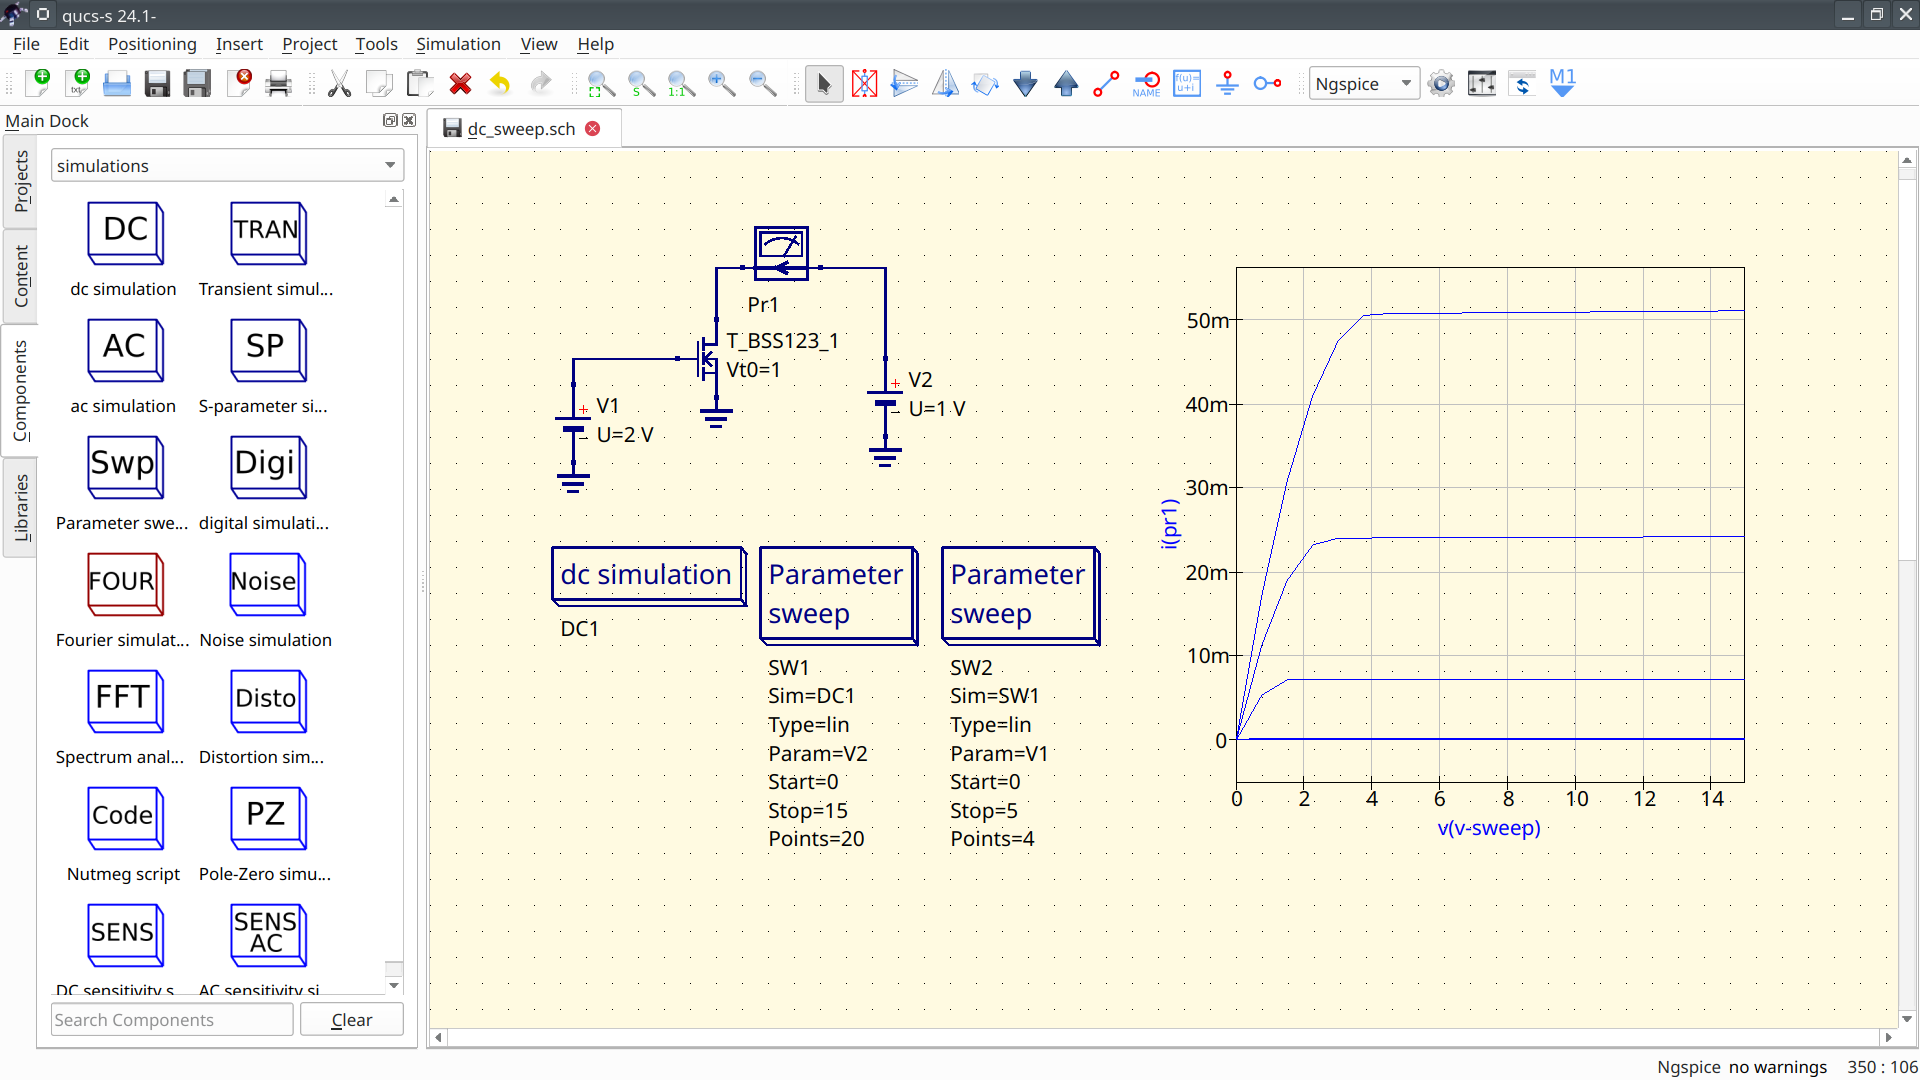
\includegraphics[width=\textwidth]{img/dc_sweep.png}
    \end{center}
    \caption{Моделирование ВАХ полевого транзистора} \label{fig:dc_sweep}
    \end{figure}

Транзистор типа BSS123 возьмём из библиотеки. К стоку и затвору подключаем два источника постоянного напряжения V1 и V2, а в цепь стока ещё и амперметр (current probe), который будет измерять ток стока. На схеме размещаем три моделирования: DC analysis и два блока Parameter Sweep. Отдельного моделирования DC sweep в Qucs-S нет, поэтому используется комбинация из двух видов моделирования. Моделирование Parameter Sweep имеет первый параметр Sim, в котором нужно указать вид моделирования. В нашем случае указываем указываем DC1, как показано на схеме. В диалоге свойств моделирования его можно выбрать из списка. В качестве параметра для развёртки (Param) указываем имя источника. В нашем случае это V2, который включён в цепь стока. В отличие от старого Qucs здесь нужно указывать только имя источника или резистора, а не имя переменной. В свойствах Start и Stop следует указать диапазон, а в свойстве Points – число точек. В нашем случае напряжения на стоке изменяется от 0 до 15 В. 

Второе моделирование Parameter Sweep нужно, чтобы получить семейство ВАХ. При этом во внутреннем цикле у нас изменяется напряжение сток-исток (источник V2), а во внешнем устанавливается напряжение на затворе (источник V1). Напряжение на затворе изменяется в пределах от 0 до 5 В.  В семействе ВАХ будет 5 кривых (Points=4). После того, как параметры моделирования заданы, можно запускать моделирования, выбрав в главном меню Simulation→ Simulate. Затем размещаем на схеме декартовскую диаграмму, на которой строим переменную i(pr1), представлявшую ток через амперметр. В результате должно получиться семейство выходных ВАХ.

\subsection{Моделирование переходных процессов}

Моделирование переходного процесса применяется, чтобы получить виртуальную осциллограмму какого-либо напряжения или тока. Данный вид моделирования называется Transient Simulation. Рассмотрим небольшой пример. Собираем схему усилителя на одном биполярном транзисторе и построим осциллограммы напряжения на входе и на выходе. Должна получиться схема, показанная на скриншоте (рис. \ref{fig:tran}).

    \begin{figure}[!ht]
    \begin{center}
        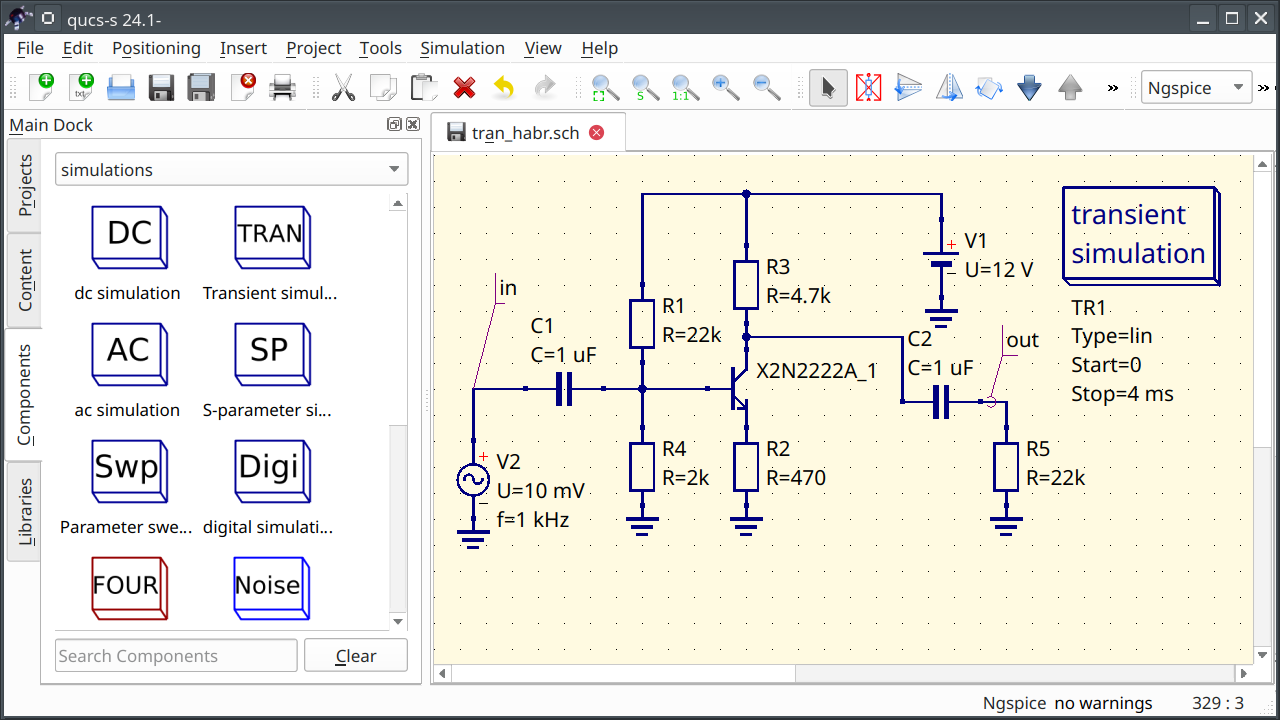
\includegraphics[width=\textwidth]{img/bjt_tran.png}
    \end{center}
    \caption{Моделирование переходных процессов} \label{fig:tran}
    \end{figure}

Транзистор типа 2N2222 можно найти в библиотеке компонентов (вкладка Library слева окна), введя его имя в строке поиска над древовидным списком библиотек. Усилитель питается от источника V1 напряжением 12В, ко входу подключен источник переменного напряжения амплитудой 100мВ и частотой 2кГц. К выходу подключена нагрузка через разделительный конденсатор. Чтобы построить осциллограммы напряжения на входе и на выходе, соответствующие узлы на схеме нужно пометить. Для этого используем кнопку Wire Label на панели инструментов. На схеме размещаем моделирование «Transient simulation». По двойному щелчку на данном компоненте открывается диалог свойств моделирования, показанный на следующем скриншоте (рис. \ref{fig:tran_set}).

    \begin{figure}[!ht]
    \begin{center}
        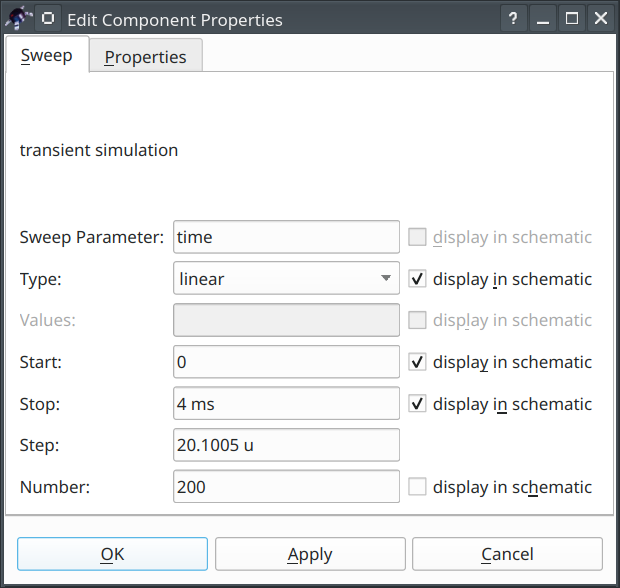
\includegraphics[width=0.4\textwidth]{img/tran_set.png}
    \end{center}
    \caption{Установки моделирования переходных процессов} \label{fig:tran_set}
    \end{figure}
    
В данном окне можно задать начальное (Start) и конечное (Stop) время, а также количество точек расчёта. В нашем случае длительность моделирования 4 мс, рассчитать требуется 200 точек, шаг расчёта около 20 мкс. Запускаем моделирование, которое должно пройти без ошибок, а затем размещаем на схему декартовскую диаграмму (Cartesian), на которой строим сигналы v(in) и v(out). Видим, что усилитель усиливает входной сигнал (рис. \ref{fig:tran_out}).

    \begin{figure}[!ht]
    \begin{center}
        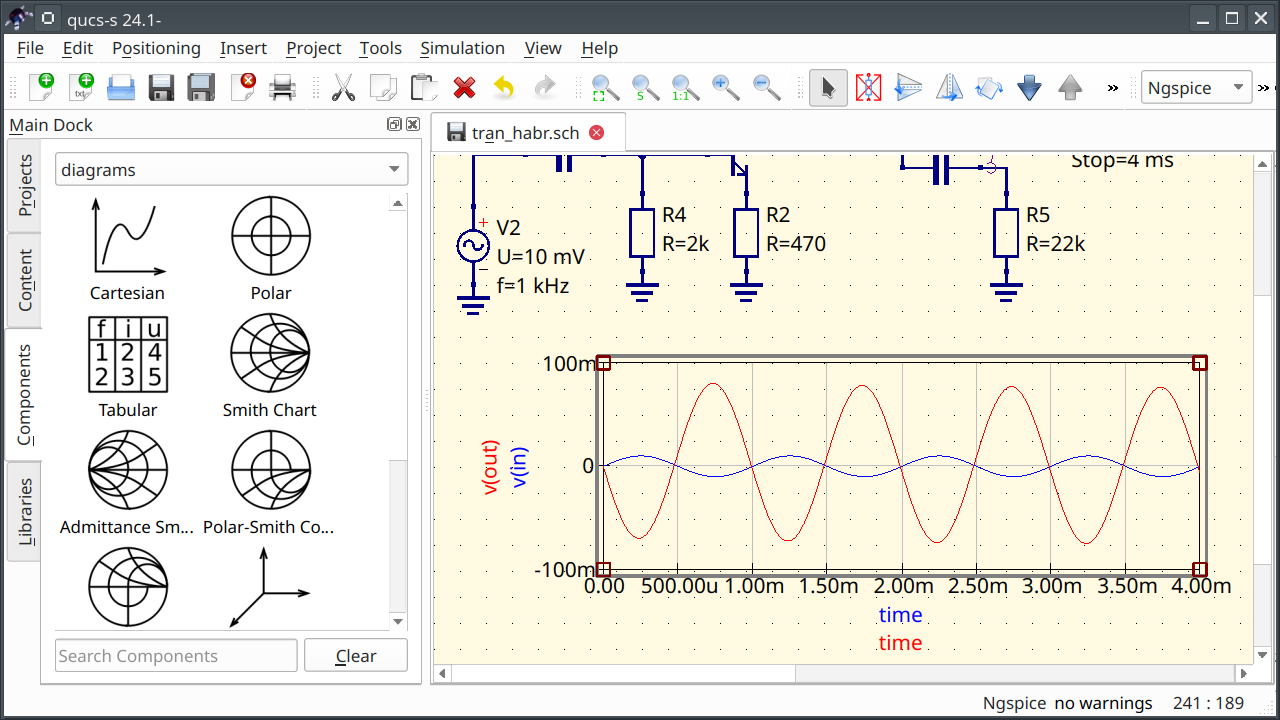
\includegraphics[width=\textwidth]{img/tran_out.png}
    \end{center}
    \caption{Результат моделирования переходных процессов} \label{fig:tran_out}
    \end{figure}

\subsection{Моделирование переходных процессов с начальными условиями}

Начальные условия для моделирования переходного процесса обычно рассчитываются автоматически. Перед началом расчёта SPICE симулятор проводит моделирование рабочей точки (initial DC) по постоянному току и из его результатов подставляет начальные условия.  Но иногда начальные условия нужно задавать вручную, например если в схеме имеются заряженные конденсаторы. Чтобы задать начальное напряжение на конденсаторах, нужно вписать значение в параметр «V», в диалоге свойств конденсатора как показано на рис. \ref{fig:cap_init}. Аналогичным способом для катушек индуктивности можно задать ток.

    \begin{figure}[!ht]
    \begin{center}
        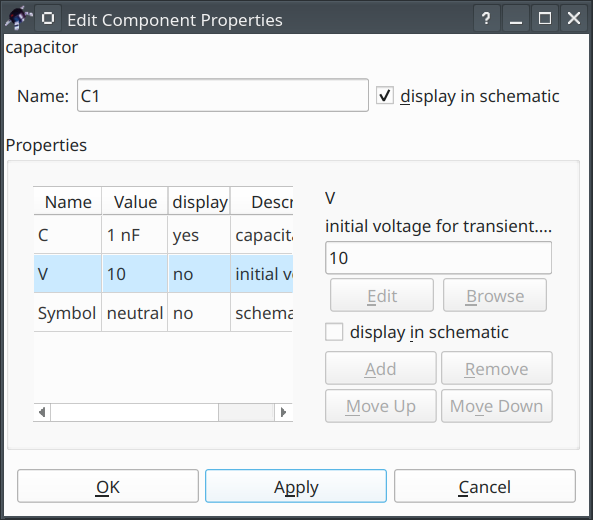
\includegraphics[width=0.4\textwidth]{img/cap_init.png}
    \end{center}
    \caption{Задание начального напряжения на конденсаторе} \label{fig:cap_init}
    \end{figure}
    
В диалоге свойств моделирования переходного процесса (рис. \ref{fig:init_dc}) следует установить параметр «inittialDC=no». По умолчанию там стоит yes. При этом отключается автоматический расчёт начальных условий.

    \begin{figure}[!ht]
    \begin{center}
        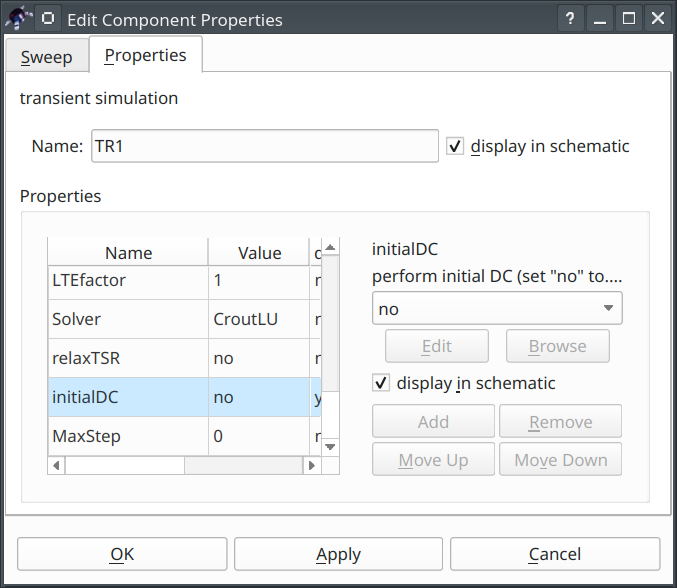
\includegraphics[width=0.4\textwidth]{img/init_dc.png}
    \end{center}
    \caption{Отключение автоматического расчёта начальных условий} \label{fig:init_dc}
    \end{figure}

В качестве примера рассмотрим схему (рис. \ref{fig:cap_discharge}), в которой моделируется разряд конденсатора. Начальное напряжение на конденсаторе задано 10В, а автоматический расчёт начальных условий отключен. В результате на узле v(cap) получаем экпоненциальную форму напряжения. Напряжение спадает от 10В до нуля по мере разряда конденсатора. Постоянная времени RC цепи в данном случае 1 мс.

    \begin{figure}[!ht]
    \begin{center}
        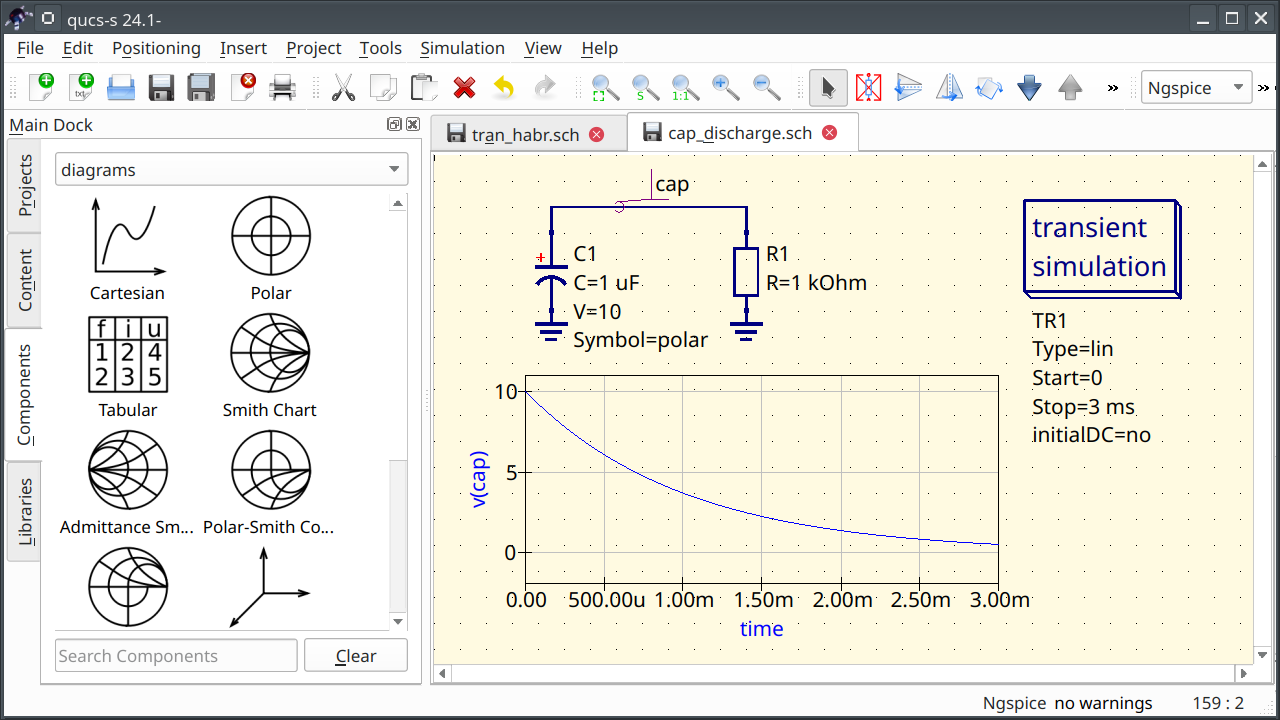
\includegraphics[width=\textwidth]{img/cap_discharge.png}
    \end{center}
    \caption{Отключение автоматического расчёта начальных условий} \label{fig:cap_discharge}
    \end{figure}

\subsection{AC analysis}

\subsection{Spectrum anylysis (FFT)}

\subsection{Fourier anylysis}

\subsection{Pole-zero anylysis}

\subsection{Distortion anylysis}

\subsection{Noise anylysis}

\subsection{Parameter sweep}

\subsection{Using tuner mode}

\subsection{Nutmeg script simulation type}

\section{RF simulation}

\subsection{RF (S-parameter) simulation with Ngspice}

\subsection{RF (S-parameter) simulation with Qucsator}

\subsection{Harmonic balance simulation with XYCE}

\subsection{Harmonic balance simulation with Qucsator}

\section{Equations and postprocessing}

\subsection{Using eqautions with Ngspice}

\subsubsection{Parameters}

\subsubsection{Nutmeg equations}

\subsection{Using equations with Qucsator}

\section{Libraries and susbcircuits}

\subsection{Library manager}

\subsection{Creating subcircuits}

\subsection{Creating libraries}

\subsection{Using SPICE models in schematics}

\subsubsection{SPICE modelcrads .MODEL}

\subsubsection{SPICE subcircuits .SUBCKT}

\section{Compact modelling}

\subsection{Using Verilog-A models with Ngspice and OpenVAF}


	
% \bibliographystyle{plain}
% \bibliography{references}
\end{document}


